%\chapter{Main Results}
\chapter{実験}

\section{モデル構成とパラメータ設定}
ネットワークにおける半教師あり学習におけるノードの分類問題のタスクにおいて実験を行った。モデルは2層のグラフ畳み込みネットワークを用い、隠れ層の活性化関数にはReLU関数、出力層の活性化関数にはソフトマックス関数を用いた。また、attention層の活性化関数にはソフトマックス関数を用いた。また、\cite{dropout}と重み減衰を用いて正則化を行った.グラフ畳み込みネットワークとattention層における重み行列は、Glorotの一様分布\cite{glorot}を用いて初期化した。最適化に用いる勾配降下法にはAdam\cite{Adam}を用いた。トレードオフパラメータ$\alpha$を用い、ラベル推測学習と構造特徴保持学習の損失を等しい割合で足し合わせたものを、最終的な目的関数として用いる.全ての実験はPython3.7で動作しており、ニューラルネットワークにおけるモデルや最適化のライブラリとしてpytorchを用いた。構造特徴の計算には、NetworkXを用いた。\\
 比較手法と平等に比較するために、ハイパーパラメータは\cite{gcn}における実験と同様の値を用いる。
 最大エポック数は200、学習率は0.01、ドロップアウト率は0.5隠れ層のサイズは32とする。また、validationセットにおける損失関数が10エポック間において減少しない場合は学習を打ち止めにするようにする。また、構造特徴は媒介中心性、近接中心性、次数中心性、固有ベクトル中心性、pagerankの5つ全てを用い実験する。
\begin{table}[h]
\begin{center}
\label{parameter}
\caption{パラメータ設定}
  \begin{tabular}{l|c} \hline
  パラメータ & 値 \\ \hline
  学習率 & 0.01 \\
  エポック数 & 200 \\
  隠れ層のユニット数 & 32 \\
  ドロップアウト率 & 0.5 \\
  重み減衰パラメータ & 5e-4\\ \hline
  %トレードオフパラメータ$\alpha$ & 0.5 \\   \hline
  \end{tabular}
  \end{center}
\end{table}

\section{データセット}
本実験で使用するデータセットはcora、citeseer、pubmedの3つであり、これらはどれも論文間の引用関係に基づいたネットワークである。これらのネットワークはノードを論文、エッジを論文の引用関係、ラベルをその論文がどの分野の論文であるかを表す。特徴ベクトルはそれぞれの論文の概要からbag of wordsを用いて、その概要に含まれる単語を抽出し表されている。データセットの概要と可視化を表\ref{dataset}と図\ref{fig:dataset}により示す.

論文の引用関係ネットワークにおいては,ノードは論文,エッジは論文の引用関係,ラベルはその論文が属する分野を表す.また,論文の概要をBag of Wordsを用いて抽出したものを特徴ベクトルとして用いている.それぞれのデータセットを可視化したものを図\ref{fig:dataset}に示す.



\begin{table}[h]
\begin{center}
\caption{データセット}
\label{dataset}
  \begin{tabular}{l|crrrrr} \hline
    &  ノード & エッジ & クラス & 特徴量  \\ \hline
    Cora & 2,708 & 5,429 & 7 & 1,433 \\
    Citeseer  & 3,327 & 4,732 & 6 & 3,703 \\
    Pubmed  & 19,717 & 44,338 & 3 & 500 \\ \hline
  \end{tabular}
  \end{center}
\end{table}

\begin{figure}%[H]
  \begin{center}
    \begin{tabular}{c}
    
    \begin{minipage}{0.5\hsize}
  \centering
  \includegraphics[width=6cm]{figures/cora.eps}
  \subcaption{Cora}
  \label{cora_vis}
\end{minipage}\\

\begin{minipage}{0.5\hsize}
  \centering
    \includegraphics[width=6cm]{figures/citeseer.eps} 
    \subcaption{Citeseer} %タイトルをつける
    \label{citeseer_vis} %ラベルをつけ図の参照を可能にする
\end{minipage}

\begin{minipage}{0.5\hsize}
  \centering
    \includegraphics[width=6cm]{figures/pubmed.eps} 
    \subcaption{Pubmed} %タイトルをつける
    \label{pubmed_vis} %ラベルをつけ図の参照を可能にする
\end{minipage}
    \end{tabular}
    \caption{各データセットの可視化}
    \label{fig:dataset}
  \end{center}
\end{figure}

\clearpage

\section{比較手法}
比較手法には、グラフ上で教師ありラベルの備わったノードから他のノードにラベルを伝搬させる手法であるラベル伝搬法(LP)\cite{LP}、ランダムウォークにより、グラフをベクトル空間に埋め込む手法であるDeepwalk\cite{DeepWalk}、サンプリングによりラベル情報とグラフを用いエンべディングを行うPlanetoid\cite{planetoid}、本研究の教師あり学習のベースとなるGCN\cite{gcn}、そのGCNに構造特徴を組み込んだ手法(GCN+ss)\cite{GCN+ss}を用いた。
ここで、GCNとGCN+ss以外の手法においては実験を行わず、\cite{gcn}で示される結果を引用する。


\section{実験結果}
\subsection{ノードの分類精度}
\ref{weakness}で述べたように、教師ありノードの割合が少ない場合は、グラフ畳みん込みネットワークにおいて、精度が大きく落ちてしまう。それにより、各データセットにおいて用いる教師データの数を各クラス数に応じて変化させることにより分類精度を比較する。教師ありノードの割合は全体のノード数に対して、Cora、Citeseerにおいては1\%,2\%,3\%,4\%,5\%、pubmedにおいては0.1\%,0.2\%,0.3\%,0.4\%,0.5\%と変化させることにより精度をそれぞれの精度を比較した。各クラスごとに等しい数の教師ありラベルを用いた。クラスごとのラベル選択により偏りがでるため、300回の実験による平均した値を分類精度とした。また、バリデーションデータとして500個、テストデータとして1000個のラベル付きデータセットを用いて評価を行った。

各データセットにおけるノード分類の精度を表\ref{cora_result} - \ref{pubmed_result}に示す。GCNを使っていない手法においては論文から引用した数値を使っているため、表の一部が空欄になっている。

\begin{table}[h]
  \begin{center}
  \caption{学習時の教師ラベル数を変化させたときの分類精度}
    \begin{tabular}{c}

      % 1
      \begin{minipage}{0.7\hsize}
        \begin{center}
     \subcaption{Coraデータセットにおける分類精度}
	\label{cora_result}
        \begin{tabular}{l|ccccc} \hline
    教師ラベル数 &  1\% & 2\% & 3\% & 4\% & 5\%  \\ \hline
    LP & -- & -- & -- & -- & 68.0 \\
    DeepWalk & -- & -- & -- & -- & 67.2 \\
    Planetoid & -- & -- & -- & -- & 75.1 \\ \hline \hline
    GCN & 67.1 & 75.0 & 77.6 & 79.5 & 80.5 \\
    GCN+SS & 68.0 & 75.4 & 78.3 & 79.8 & 80.8 \\
    {\bf Proposed} & 68.8 & 75.8 & 78.0 & 79.8 & 80.8 \\ \hline
  \end{tabular}
        \end{center}
             \vspace{1cm}
      \end{minipage}\\
      
 
      
      % 2
      \begin{minipage}{0.7\hsize}
        \begin{center}
    \subcaption{Citeseerデータセットにおける分類精度}
\label{citeseer_result}
  \begin{tabular}{l|ccccc} \hline
    教師ラベル数 &  1\% & 2\% & 3\% & 4\% & 5\%  \\ \hline
     LP & -- & -- & -- & -- & 45.3 \\
    DeepWalk & -- & -- & -- & -- & 43.2 \\
    Planetoid & -- & -- & -- & -- & 64.7 \\ \hline \hline
    GCN & 60.4 & 66.3 & 68.3 & 69.5 & 70.2 \\
    GCN+SS & 62.0 & 67.3 & 68.8 & 69.9 & 70.5 \\
    {\bf Proposed} & 62.1 & 66.8 & 68.8 & 69.7 & 70.5 \\ \hline
  \end{tabular}
        \end{center}
          \vspace{1cm}
      \end{minipage}\\
      
    
      
          \begin{minipage}{0.7\hsize}
        \begin{center}
    \subcaption{Pubmedデータセットにおける分類精度}
\label{pubmed_result}
  \begin{tabular}{l|ccccc} \hline
    教師ラベル数 &  0.1\% & 0.2\% & 0.3\% & 0.4\% & 0.5\%  \\ \hline
     LP & -- & -- & -- & -- & 63.0 \\
    DeepWalk & -- & -- & -- & -- & 65.3 \\
    Planetoid & -- & -- & -- & -- & 77.2 \\ \hline \hline
    GCN & 71.0 & 75.5 & 77.5 & 78.8 & 79.8 \\
    GCN+SS & 71.8 & 75.4 & 77.3 & 78.2 & - \\
    {\bf Proposed} & 71.4 & 75.1 & 77.1 & 78.6 & 79.5 \\ \hline
  \end{tabular}
        \end{center}
      \end{minipage}

    \end{tabular}
  \end{center}
\end{table}



それぞれのデータセットにおける分類精度を評価したものを表\ref{cora_result} - \ref{pubmed_result}に示す.教師ラベル数とは,全てのノードのうちラベル付けされているノードの割合を表す.GCN以外の比較手法については,論文から引用した数値を用いたため,空欄となっている箇所がある.また,GCNと提案手法の精度を比較したグラフを図\ref{fig:cora_result} - \ref{fig:pubmed_result}に示す.横軸は学習データサイズ,縦軸は分類精度を表す.
全てのデータセットにおいて,提案手法が最も高い精度を示している.とくに,教師ラベルの数が少ない場合において,提案手法は既存手法よりも大きく精度が向上している.これは,教師ラベルが少ない場合には,構造特徴を用いることで,学習時の情報の少なさを補っているためだと考えられる.









\subsection{トレードオフパラメータの$\alpha$による推移}
提案手法においてはトレードオフパラメータ$\alpha$を用いて、教師ありの損失と教師なしの損失の重み付けをしている。このパラメータによりどれほど影響がでるかを調べるために実験を行った。attentionメカニズムを用いずに構造特徴を均等に教師なし学習させたモデルであるGCN\_ssと構造特徴にattentionメカニズムを組み込んだ提案手法を比較した。実験はハイパーパラメータ$\alpha$を0から1まで0.1刻みで値を変化させ、それぞれのデータセットにおいてそれぞれの$\alpha$で300回の施行を行い、精度の比較を行った。教師データの数はcora,citeseer,pubmedで各ラベルの種類ごとに4,7,6個(全体における1\%、1\%、0.1\%)用い、結果は図\ref{cora_alpha}、図\ref{citeseer_alpha}、図\ref{pubmed_alpha}のようになった。横軸はハイパーパラメータ$\alpha$、縦軸はノードの分類精度を表している。図から分かるように、$\alpha$=1に近い場合、分類精度が大きく低下しているが、これは構造特徴を用いた精度教師なし学習による学習の比率がほとんどを占めるため精度落ちていると推測できる。coraやciteseerにおいては$\alpha$=0の場合は構造特徴による学習がされていなく、精度が落ちていると考えられる。

\begin{figure*}[h]
  \centering
    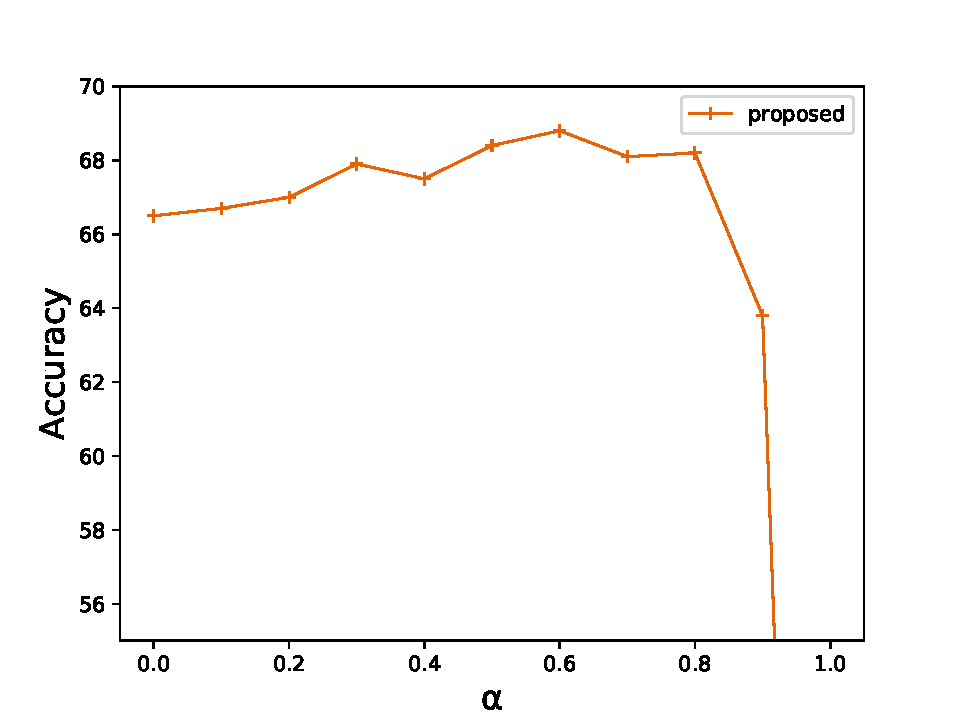
\includegraphics[width=12cm]{figures/cora_solo.pdf}
     \vspace*{0.5cm} 
    \caption{coraにおける比較} %タイトルをつける
    \label{cora_alpha} %ラベルをつけ図の参照を可能にする
\end{figure*}

\begin{figure*}[h]
  \centering
    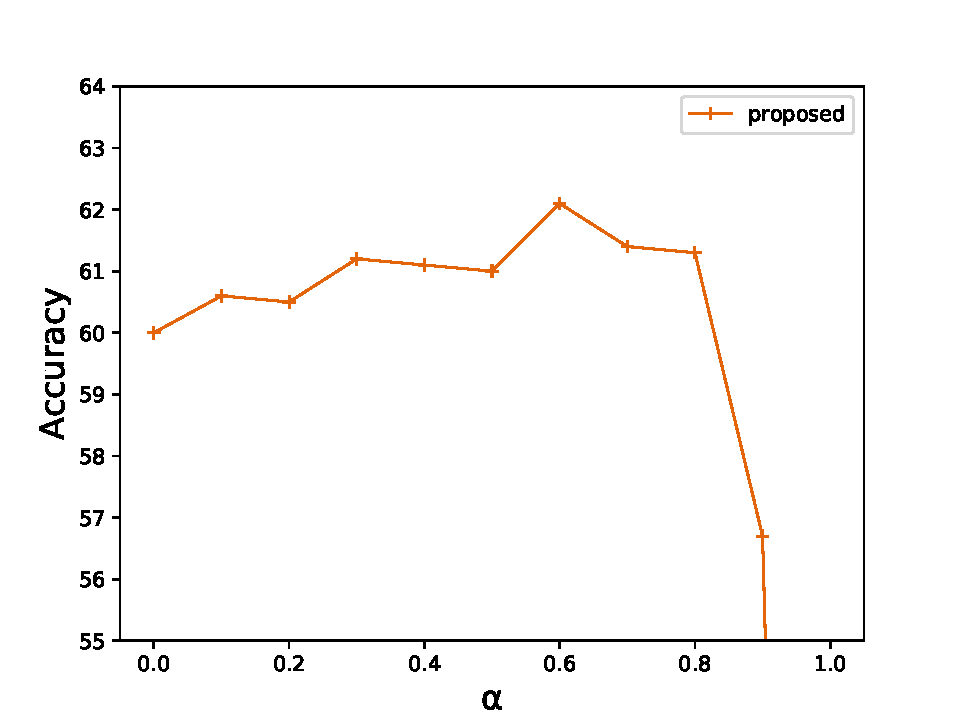
\includegraphics[width=12cm]{figures/citeseer_solo.pdf}
     \vspace*{0.5cm} 
    \caption{citeseerにおける比較} %タイトルをつける
    \label{citeseer_alpha} %ラベルをつけ図の参照を可能にする
\end{figure*}

\begin{figure*}[h]
  \centering
    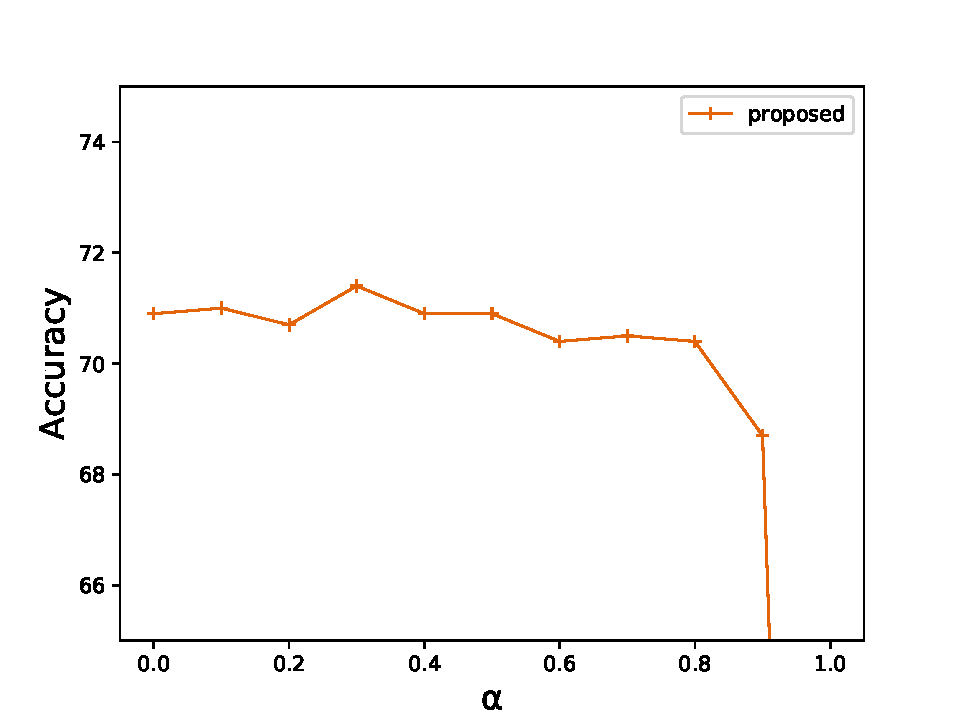
\includegraphics[width=12cm]{figures/pubmed_solo.pdf}
     \vspace*{0.5cm} 
    \caption{pubmedにおける比較} %タイトルをつける
    \label{pubmed_alpha} %ラベルをつけ図の参照を可能にする
\end{figure*}


